\section{講義概要}


\begin{frame}
\frametitle{今日の内容}



\begin{enumerate}
\item 平均変化率, 微分係数, 接線の傾き
\item 導関数, 導関数の性質
\end{enumerate} 



\end{frame}





%%%%%%%%%%%%%%%%%%%%%%%%%%%%%%%%%%%%%%%%%%%%%%%%%%%%%%%%%%%%%%%%%%%%%%%%%%%%%%%%%%%%%%%
%%%%%%%%%%%%%%%%%%%%%%%%%%%%%%%%%%%%%%%%%%%%%%%%%%%%%%%%%%%%%%%%%%%%%%%%%%%%%%%%%%%%%%%

\section{極限の別表記}


\begin{frame}
\frametitle{極限の別表示}


前回, 関数$f(x)$の$a$における極限を,
$$
\lim_{x \to a +0}f(x)=\lim_{x \to a -0}f(x)=\alpha
$$
であるときに, $\displaystyle \lim_{x \to a}f(x)=\alpha$と定義した. \\
\ \\

上記の条件は, $x=a+h$と表すと, 
$$
\lim_{h \to +0}f(a+h)=\lim_{h\to -0}f(a+h)=\alpha
$$
と同値であり, これを$\displaystyle \lim_{h \to 0}f(a+h)=\alpha$と書く. 
今回の講義では後者の表記を用いる. 


\end{frame}



%%%%%%%%%%%%%%%%%%%%%%%%%%%%%%%%%%%%%%%%%%%%%%%%%%%%%%%%%%%%%%%%%%%%%%%%%%%%%%%%%%%%%%%
%%%%%%%%%%%%%%%%%%%%%%%%%%%%%%%%%%%%%%%%%%%%%%%%%%%%%%%%%%%%%%%%%%%%%%%%%%%%%%%%%%%%%%%

\section{平均変化率}

\begin{frame}
\frametitle{平均変化率}

\vspace{-5mm}

 \begin{figure}[htbp]
 \begin{center} 
  
\includegraphics[width=75mm]{calculus4/600km.png}
 \end{center}
\end{figure}

\vspace{-5mm}

\begin{Prob}
$600$kmの移動に$3$時間かかったとき, 速度は何km/hだろうか?
\end{Prob}

答えは簡単で, 
$$
\frac{\text{$600$km}}{\text{$3$時間}}=200\text{km/h}
$$
と答えたくなる. \\
\ \\

しかしながら, これは平均速度であり, 常に一定の速度で移動するとは限らない. 
つまり, ある特定の時刻での速度は必ずしも$200$km/hになるとは限らない. \\
\ \\

この問題設定からは, 平均速度しか求めることができない. 

\end{frame}





%%%%%%%%%%%%%%%%%%%%%%%%%%%%%%%%%%%%%%%%%%%%%%%%%%%%%%%%%%%%%%%%%%%%%%%%%%%%%%%%%%%%%%%
%%%%%%%%%%%%%%%%%%%%%%%%%%%%%%%%%%%%%%%%%%%%%%%%%%%%%%%%%%%%%%%%%%%%%%%%%%%%%%%%%%%%%%%


\begin{frame}
\frametitle{平均変化率}

出発からちょうど$1$時間後の速度はどのように求めれば良いだろうか? 

\vspace{-2mm}

 \begin{figure}[htbp]
 \begin{center} 
  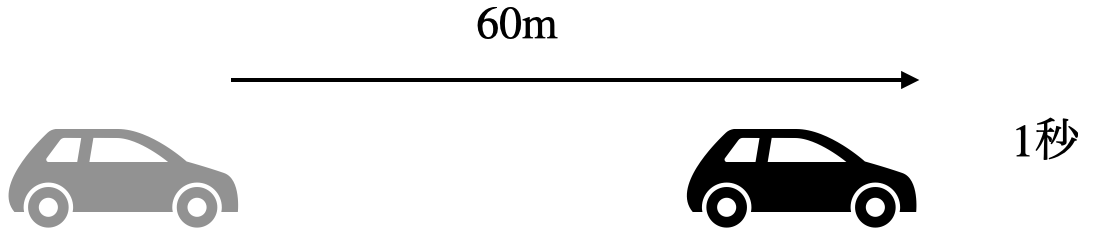
\includegraphics[width=55mm]{calculus4/60m.png}
 \end{center}
\end{figure}

\vspace{-2mm}

出発してから$1$時間後において, $1$秒間で$60$m移動したとすると, 
$$
\frac{\text{$60$m}}{\text{$1$秒}}=
\frac{\text{$0.06$km}}{\text{$1/3600$時間}}=216\text{km/h}
$$
と答えたくなる. \\
\ \\

しかしながら, 時間スケールを変えただけで, 状況は先の問題と変わっていない. 
これは$1$秒間の平均速度であり, 
$1$秒間の間に速度が変化している可能性がある. 


\end{frame}




%%%%%%%%%%%%%%%%%%%%%%%%%%%%%%%%%%%%%%%%%%%%%%%%%%%%%%%%%%%%%%%%%%%%%%%%%%%%%%%%%%%%%%%
%%%%%%%%%%%%%%%%%%%%%%%%%%%%%%%%%%%%%%%%%%%%%%%%%%%%%%%%%%%%%%%%%%%%%%%%%%%%%%%%%%%%%%%


\begin{frame}
\frametitle{平均変化率}

\vspace{-10mm}

 \begin{figure}[htbp]
 \begin{center} 
  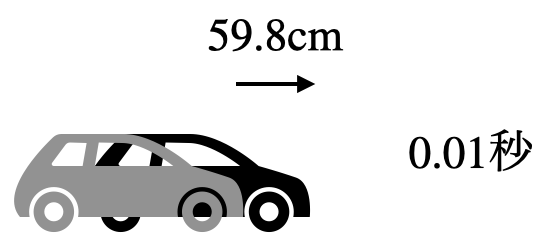
\includegraphics[width=30mm]{calculus4/59cm.png}
 \end{center}
\end{figure}

\vspace{-2mm}

時間をさらに細かく刻んで$0.01$秒間にどれだけ移動したかを計測したところ, $59.8$cm移動したことが判明した. 
するとこの$0.01$秒間の平均速度は
$$
\frac{\text{$59.8$cm}}{\text{$0.01$秒}}=
\frac{\text{$0.000598$km}}{\text{$1/360000$時間}}=215.28\text{km/h}
$$
となる. \\
\ \\

もちろんこの$0.01$秒間の間に速度が変化している可能性があるが, 良い近似になっていることが期待される.  


\end{frame}



%%%%%%%%%%%%%%%%%%%%%%%%%%%%%%%%%%%%%%%%%%%%%%%%%%%%%%%%%%%%%%%%%%%%%%%%%%%%%%%%%%%%%%%
%%%%%%%%%%%%%%%%%%%%%%%%%%%%%%%%%%%%%%%%%%%%%%%%%%%%%%%%%%%%%%%%%%%%%%%%%%%%%%%%%%%%%%%


\begin{frame}
\frametitle{平均変化率}


一般に, 時間軸をどんどん短くすることで, その時刻での速度をより正確に測定できることが期待される.\\
\ \\

つまり, ある時刻での速度は
$$
\frac{\text{微小な位置の変化}}{\text{微小な時間の変化}}
$$
の極限として得られると考えられる. \\
%ここで微小な時間の変化とは, さらに分割できないほど短い時間スケールのことである.  \\
\ \\

このような極限を扱う理論が微分である. 


\end{frame}


%%%%%%%%%%%%%%%%%%%%%%%%%%%%%%%%%%%%%%%%%%%%%%%%%%%%%%%%%%%%%%%%%%%%%%%%%%%%%%%%%%%%%%%
%%%%%%%%%%%%%%%%%%%%%%%%%%%%%%%%%%%%%%%%%%%%%%%%%%%%%%%%%%%%%%%%%%%%%%%%%%%%%%%%%%%%%%%

\section{微分係数}

\begin{frame}
\frametitle{微分係数}

\begin{Def}
関数$f(x)$の定義域を$D$とする. 
点$a \in D$に関して, 極限
$$
\lim_{h\to 0} \frac{f(a+h)-f(a)}{h}
$$
が存在するとき, $f(x)$は$a$で\underline{微分可能}であるといい, $f'(a)$で表す. 
$f'(a)$は$f(x)$の$a$における\underline{微分係数}と呼ばれる. 
\end{Def}

$f(x)$は$a$で微分可能ならば, $f(x)$は$a$で連続であることがわかるが, その逆は一般には成立しない. 


\end{frame}


%%%%%%%%%%%%%%%%%%%%%%%%%%%%%%%%%%%%%%%%%%%%%%%%%%%%%%%%%%%%%%%%%%%%%%%%%%%%%%%%%%%%%%%
%%%%%%%%%%%%%%%%%%%%%%%%%%%%%%%%%%%%%%%%%%%%%%%%%%%%%%%%%%%%%%%%%%%%%%%%%%%%%%%%%%%%%%%


\begin{frame}
\frametitle{微分係数と接線の傾き}

微分係数
$$
f'(a)=
\lim_{h\to 0} \frac{f(a+h)-f(a)}{h}
$$
は$f(x)$のグラフの点$(a,f(a))$における接線の傾きとみなすことができる. 
 

 \begin{figure}[htbp]
 \begin{center} 
  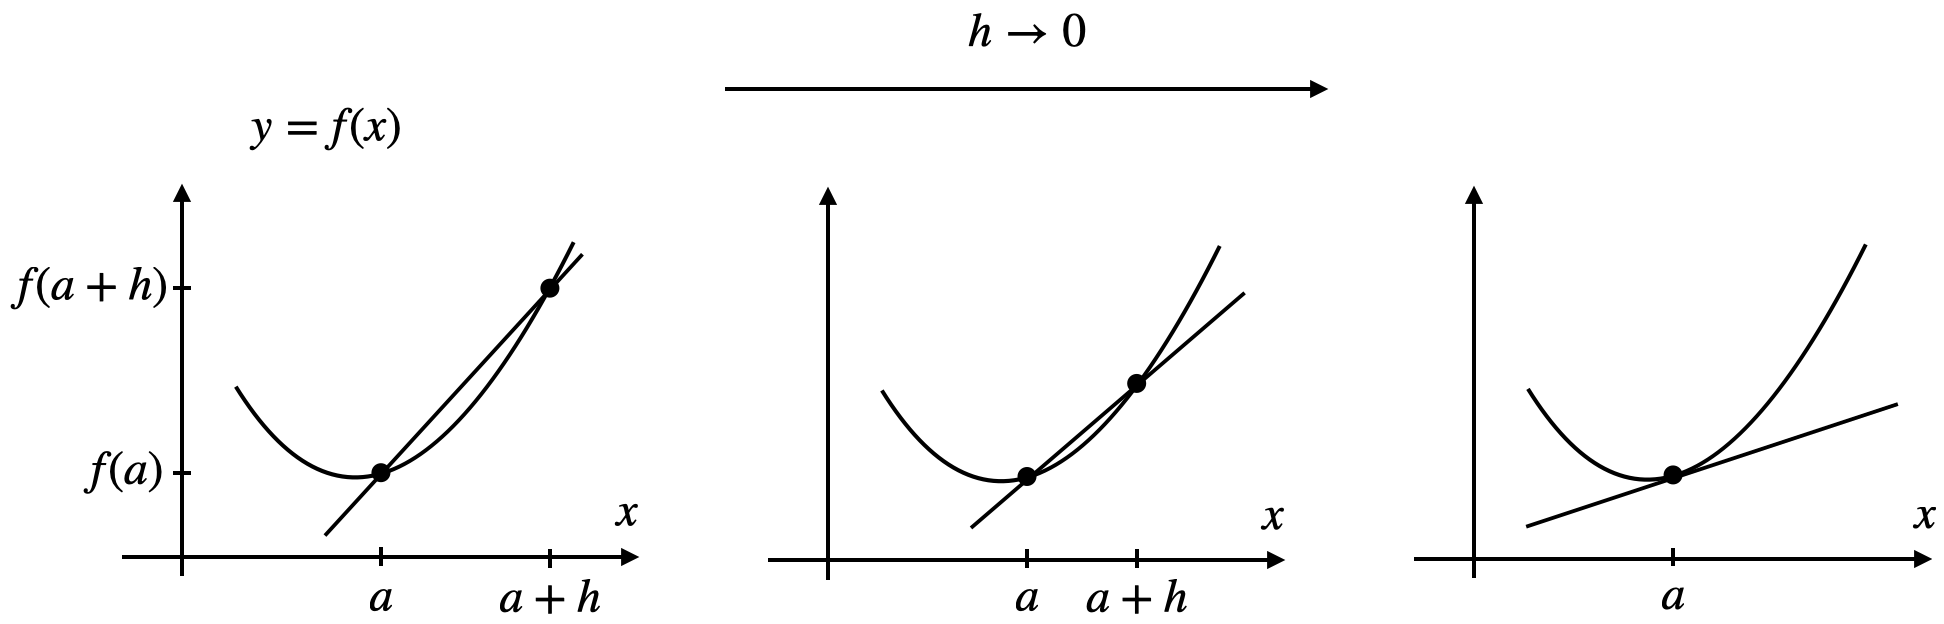
\includegraphics[width=120mm]{calculus4/tangent.png}
 \end{center}
\end{figure}


\end{frame}

%%%%%%%%%%%%%%%%%%%%%%%%%%%%%%%%%%%%%%%%%%%%%%%%%%%%%%%%%%%%%%%%%%%%%%%%%%%%%%%%%%%%%%%
%%%%%%%%%%%%%%%%%%%%%%%%%%%%%%%%%%%%%%%%%%%%%%%%%%%%%%%%%%%%%%%%%%%%%%%%%%%%%%%%%%%%%%%

\begin{frame}
\frametitle{微分可能性}

関数$f(x)$が$a$において微分可能であるとは, $f(x)$のグラフが点$(a,f(a))$における接線が定義できるくらい滑らかであることを意味する. 
点$(a,f(a))$の近傍でグラフが直線のように見えるともいえる.  
%この直線の傾きが$f'(a)$である. 


 \begin{figure}[htbp]
 \begin{center} 
  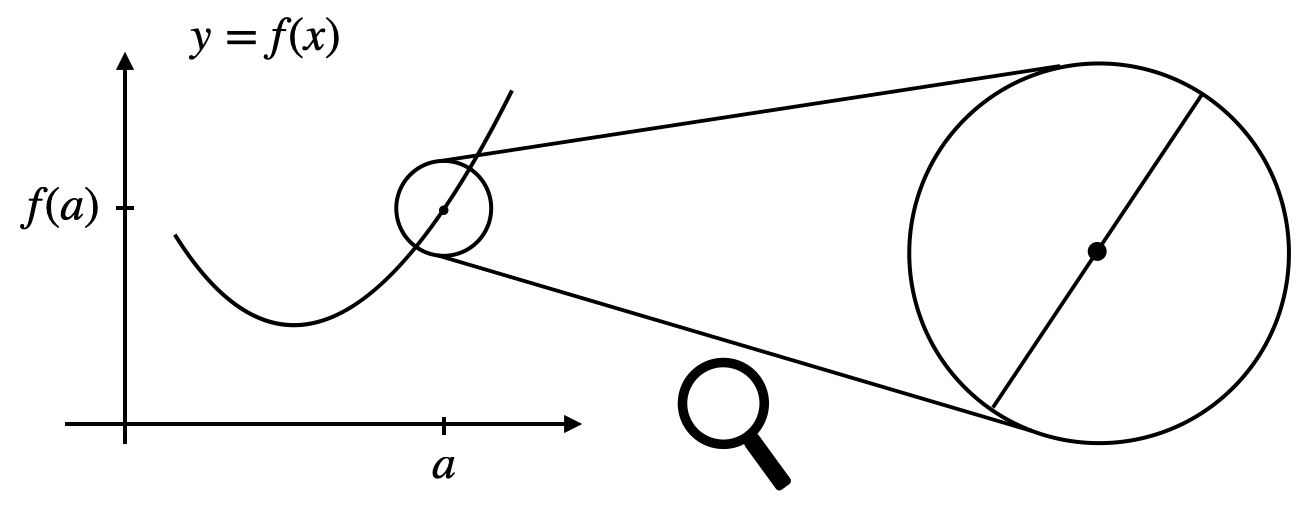
\includegraphics[width=85mm]{calculus4/differentiable2.png}
 \end{center}
\end{figure}

\end{frame}



%%%%%%%%%%%%%%%%%%%%%%%%%%%%%%%%%%%%%%%%%%%%%%%%%%%%%%%%%%%%%%%%%%%%%%%%%%%%%%%%%%%%%%%
%%%%%%%%%%%%%%%%%%%%%%%%%%%%%%%%%%%%%%%%%%%%%%%%%%%%%%%%%%%%%%%%%%%%%%%%%%%%%%%%%%%%%%

\section{導関数}

\begin{frame}
\frametitle{導関数}


\begin{Def}
関数$f(x)$がその定義域$D$の任意の点において微分可能であるとする. 
$a \in D$に対して, その点における微分係数$f'(a)$を返す関数
$$
f':D \longrightarrow \R, \ \ \ a \to f'(a)
$$
を$f(x)$の\underline{導関数}と呼び, $f'(x)$を求める事を$f(x)$を\underline{微分する}という.  
$f'(x)$は$\frac{df}{dx}(x)$と書かれる場合もある. 
\end{Def}

\end{frame}



%%%%%%%%%%%%%%%%%%%%%%%%%%%%%%%%%%%%%%%%%%%%%%%%%%%%%%%%%%%%%%%%%%%%%%%%%%%%%%%%%%%%%%%
%%%%%%%%%%%%%%%%%%%%%%%%%%%%%%%%%%%%%%%%%%%%%%%%%%%%%%%%%%%%%%%%%%%%%%%%%%%%%%%%%%%%%%

\begin{frame}
\frametitle{$(x)'=1$}


$f(x)=x$の導関数を定義に従って計算する. 
\begin{align*}
f'(x) & = \lim_{h\to 0} \frac{(x+h)-x}{h} \\
& =  \lim_{h\to 0} \frac{h}{h} \\
& =  \lim_{h\to 0} 1=1. 
\end{align*}

``$f(x)=x$のグラフの点$(a,a)$における接線の傾きは$1$." 

\end{frame}



%%%%%%%%%%%%%%%%%%%%%%%%%%%%%%%%%%%%%%%%%%%%%%%%%%%%%%%%%%%%%%%%%%%%%%%%%%%%%%%%%%%%%%%
%%%%%%%%%%%%%%%%%%%%%%%%%%%%%%%%%%%%%%%%%%%%%%%%%%%%%%%%%%%%%%%%%%%%%%%%%%%%%%%%%%%%%%

\begin{frame}
\frametitle{$(x^2)'=2x$}


$f(x)=x^2$の導関数を定義に従って計算する. 
\begin{align*}
f'(x) & = \lim_{h\to 0} \frac{(x+h)^2-x^2}{h} \\
& =  \lim_{h\to 0} \frac{x^2+2hx+h^2-x^2}{h} \\
& =  \lim_{h\to 0} \frac{2hx+h^2}{h} \\
& =  \lim_{h\to 0} (2x+h) =2x. 
\end{align*}

``$f(x)=x^2$のグラフの点$(a,a^2)$における接線の傾きは$2a$." 

\end{frame}



%%%%%%%%%%%%%%%%%%%%%%%%%%%%%%%%%%%%%%%%%%%%%%%%%%%%%%%%%%%%%%%%%%%%%%%%%%%%%%%%%%%%%%%
%%%%%%%%%%%%%%%%%%%%%%%%%%%%%%%%%%%%%%%%%%%%%%%%%%%%%%%%%%%%%%%%%%%%%%%%%%%%%%%%%%%%%%

\begin{frame}
\frametitle{$(x^3)'=? $}


\begin{Prob}
$f(x)=x^3$の導関数を定義に従って計算せよ. 
つまり
$$
f'(x)  = \lim_{h\to 0} \frac{(x+h)^3-x^3}{h}
$$
を求めよ. 
\end{Prob}

\end{frame}



%%%%%%%%%%%%%%%%%%%%%%%%%%%%%%%%%%%%%%%%%%%%%%%%%%%%%%%%%%%%%%%%%%%%%%%%%%%%%%%%%%%%%%%
%%%%%%%%%%%%%%%%%%%%%%%%%%%%%%%%%%%%%%%%%%%%%%%%%%%%%%%%%%%%%%%%%%%%%%%%%%%%%%%%%%%%%%


\begin{frame}
\frametitle{$(x^3)'=3x^2$}


$f(x)=x^3$の導関数を定義に従って計算する. 
\begin{align*}
f'(x) & = \lim_{h\to 0} \frac{(x+h)^3-x^3}{h} \\
& =  \lim_{h\to 0} \frac{x^3+3hx^2+3h^2x+h^3-x^3}{h} \\
& =  \lim_{h\to 0} \frac{3hx^2+3h^2x+h^3}{h} \\
& =  \lim_{h\to 0} (3x^2+3hx+h^2) =3x^2. 
\end{align*}

``$f(x)=x^3$のグラフの点$(a,a^3)$における接線の傾きは$3a^2$." 

\end{frame}


%%%%%%%%%%%%%%%%%%%%%%%%%%%%%%%%%%%%%%%%%%%%%%%%%%%%%%%%%%%%%%%%%%%%%%%%%%%%%%%%%%%%%%%
%%%%%%%%%%%%%%%%%%%%%%%%%%%%%%%%%%%%%%%%%%%%%%%%%%%%%%%%%%%%%%%%%%%%%%%%%%%%%%%%%%%%%%


\begin{frame}
\frametitle{$(x^n)'=nx^{n-1}$}

$n \in \N$に関して, $f(x)=x^n$の導関数を定義に従って計算する. 
\begin{align*}
f'(x) & = \lim_{h\to 0} \frac{(x+h)^n-x^n}{h} \\
& =  \lim_{h\to 0} \frac{x^n+nhx^{n-1}+\frac{n(n-1)}{2}h^2x^{n-2}+\dots+h^n-x^n}{h} \\
& =  \lim_{h\to 0} \frac{nhx^{n-1}+\frac{n(n-1)}{2}h^2x^{n-2}+\dots+h^n}{h} \\
& =  \lim_{h\to 0} (nx^{n-1}+\frac{n(n-1)}{2}hx^{n-2}+\dots+h^{n-1}) =nx^{n-1}.  
\end{align*}

``$f(x)=x^n$のグラフの点$(a,a^n)$における接線の傾きは$na^{n-1}$." 

\end{frame}


%%%%%%%%%%%%%%%%%%%%%%%%%%%%%%%%%%%%%%%%%%%%%%%%%%%%%%%%%%%%%%%%%%%%%%%%%%%%%%%%%%%%%%%
%%%%%%%%%%%%%%%%%%%%%%%%%%%%%%%%%%%%%%%%%%%%%%%%%%%%%%%%%%%%%%%%%%%%%%%%%%%%%%%%%%%%%%


\begin{frame}
\frametitle{$c'=0$}

定数関数$f(x)=c$の導関数を定義に従って計算する. 
\begin{align*}
f'(x) & = \lim_{h\to 0} \frac{c-c}{h} \\
& = \lim_{h\to 0}\frac{0}{h}=0
\end{align*}

``$f(x)=c$のグラフの点$(a,c)$における接線の傾きは$0$." 

\end{frame}



%%%%%%%%%%%%%%%%%%%%%%%%%%%%%%%%%%%%%%%%%%%%%%%%%%%%%%%%%%%%%%%%%%%%%%%%%%%%%%%%%%%%%%%
%%%%%%%%%%%%%%%%%%%%%%%%%%%%%%%%%%%%%%%%%%%%%%%%%%%%%%%%%%%%%%%%%%%%%%%%%%%%%%%%%%%%%%


\begin{frame}
\frametitle{微分の性質}

\begin{Thm} \label{微分定理}
$f(x)$, $g(x)$を(共通の定義域で)微分可能な関数とする. \vspace{1mm}
\begin{enumerate}
\item $(af(x)+bg(x))'=af'(x)+bg'(x)$ \ \ \ $a,b \in \R$, \vspace{1mm}
\item $(f(x)g(x))'=f'(x)g(x)+f(x)g'(x)$, \vspace{1mm}
\item $\Big(\frac{f(x)}{g(x)}\Big)'=\frac{f'(x)g(x)-f(x)g'(x)}{g(x)^2}$
\end{enumerate}
\end{Thm}
これから
$$
(f(x)^2)'=2f'(x)f(x), \ \ \ \Big(\frac{1}{g(x)}\Big)'=-\frac{g'(x)}{g(x)^2}
$$
などが分かる. 

\end{frame}




%%%%%%%%%%%%%%%%%%%%%%%%%%%%%%%%%%%%%%%%%%%%%%%%%%%%%%%%%%%%%%%%%%%%%%%%%%%%%%%%%%%%%%%
%%%%%%%%%%%%%%%%%%%%%%%%%%%%%%%%%%%%%%%%%%%%%%%%%%%%%%%%%%%%%%%%%%%%%%%%%%%%%%%%%%%%%%


\begin{frame}
\frametitle{多項式の微分}

定理\ref{微分定理}を使うと, 多項式の導関数は簡単に計算できる.  

\begin{itemize}
\item $(3x^2-5x+1)'=6x-5$, 
\item $(x^4-15x^2+5x+\pi)'=4x^3-30x+5$, 
\item $(-x^{100}+57x^{2}+\pi x+ \log_2 7)'=-100x^{99}+114x+\pi$. 
\end{itemize}

関数のグラフが描けなくても, 接線の傾きはすぐ分かる. 

\end{frame}

%%%%%%%%%%%%%%%%%%%%%%%%%%%%%%%%%%%%%%%%%%%%%%%%%%%%%%%%%%%%%%%%%%%%%%%%%%%%%%%%%%%%%%%
%%%%%%%%%%%%%%%%%%%%%%%%%%%%%%%%%%%%%%%%%%%%%%%%%%%%%%%%%%%%%%%%%%%%%%%%%%%%%%%%%%%%%%


\begin{frame}
\frametitle{積の微分}

$(x^3+5)(4x+1)$の導関数を2通りの方法で計算する. 

\begin{itemize}
\item 定理\ref{微分定理}を使うと
\begin{align*}
\big((x^3+5)(4x+1)\big)'&=(x^3+5)'(4x+1)+(x^3+5)(4x+1)' \\
&= 3x^2(4x+1)+(x^3+5)4 \\
&= 16x^3+3x^2+20. 
\end{align*}
\item 微分の計算の前に展開すれば
\begin{align*}
\big((x^3+5)(4x+1)\big)'&= \big(4x^4+x^3+20x+5\big)' \\
&= 16x^3+3x^2+20. 
\end{align*}
\end{itemize}

\end{frame}



%%%%%%%%%%%%%%%%%%%%%%%%%%%%%%%%%%%%%%%%%%%%%%%%%%%%%%%%%%%%%%%%%%%%%%%%%%%%%%%%%%%%%%%
%%%%%%%%%%%%%%%%%%%%%%%%%%%%%%%%%%%%%%%%%%%%%%%%%%%%%%%%%%%%%%%%%%%%%%%%%%%%%%%%%%%%%%


\begin{frame}
\frametitle{商の微分}

定理\ref{微分定理}の関数の商の微分公式
$$
\Big(\frac{f(x)}{g(x)}\Big)'=\frac{f'(x)g(x)-f(x)g'(x)}{g(x)^2}
$$
を思い出す. \\
\ \\

有理関数$\frac{3x}{x^2+1}$の導関数は
\begin{align*}
\Big(\frac{3x}{x^2+1}\Big)' &= \frac{(3x)'(x^2+1)-3x(x^2+1)'}{(x^2+1)^2} \\
& = \frac{3(x^2+1)-3x(2x)}{(x^2+1)^2} \\
&=  \frac{3(-x^2+1)}{(x^2+1)^2}. 
\end{align*}


\end{frame}


%%%%%%%%%%%%%%%%%%%%%%%%%%%%%%%%%%%%%%%%%%%%%%%%%%%%%%%%%%%%%%%%%%%%%%%%%%%%%%%%%%%%%%%
%%%%%%%%%%%%%%%%%%%%%%%%%%%%%%%%%%%%%%%%%%%%%%%%%%%%%%%%%%%%%%%%%%%%%%%%%%%%%%%%%%%%%%


\begin{frame}
\frametitle{$(1/x^n)'=-n/x^{n+1}$}

逆数の微分公式
$$
\Big(\frac{1}{g(x)}\Big)'=-\frac{g'(x)}{g(x)^2}
$$
を思い出す. \\
\ \\

有理関数$\frac{1}{x^n}$の導関数は
\begin{align*}
\Big(\frac{1}{x^n}\Big)' = -\frac{(x^n)'}{(x^n)^2}=-\frac{nx^{n-1}}{x^{2n}}=\frac{-n}{x^{n+1}}. 
\end{align*}
これより
$$
(x^n)'=nx^{n-1}
$$
は任意の$n \in \Z$に対して成立することが分かる. 

\end{frame}



%%%%%%%%%%%%%%%%%%%%%%%%%%%%%%%%%%%%%%%%%%%%%%%%%%%%%%%%%%%%%%%%%%%%%%%%%%%%%%%%%%%%%%%
%%%%%%%%%%%%%%%%%%%%%%%%%%%%%%%%%%%%%%%%%%%%%%%%%%%%%%%%%%%%%%%%%%%%%%%%%%%%%%%%%%%%%%


\begin{frame}
\frametitle{微分可能 $\Rightarrow$ 連続}

関数$f(x)$は「$a$で微分可能であれば, 連続である」. 
実際, 
\begin{align*}
& \lim_{h\to 0} \frac{f(a+h)-f(a)}{h} \  \text{が有限の値として存在}\\ 
\Longrightarrow & \lim_{h\to 0} \big(f(a+h)-f(a)\big)=0 \\
\Longrightarrow &  \lim_{h\to 0} f(a+h)= f(a) \\
\Longrightarrow & \text{$\lim_{ x \to a} f(x)$が存在してその値が$f(a)$と一致} \\
\Longrightarrow & \text{$f(x)$が$x=a$で連続}
\end{align*}
対偶を考えれば, 「$a$で連続でなければ, 微分可能でない」とも表現できる.  


\end{frame}


%%%%%%%%%%%%%%%%%%%%%%%%%%%%%%%%%%%%%%%%%%%%%%%%%%%%%%%%%%%%%%%%%%%%%%%%%%%%%%%%%%%%%%%
%%%%%%%%%%%%%%%%%%%%%%%%%%%%%%%%%%%%%%%%%%%%%%%%%%%%%%%%%%%%%%%%%%%%%%%%%%%%%%%%%%%%%%


\begin{frame}
\frametitle{導関数の非存在}

関数$f(x)$は$a$で連続でなければ微分可能でないが, 連続であっても微分可能とは限らない. \\
\ \\

例えば, $f(x)=|x|$は$0$で微分不可能である. 

 \begin{figure}[htbp]
 \begin{center} 
  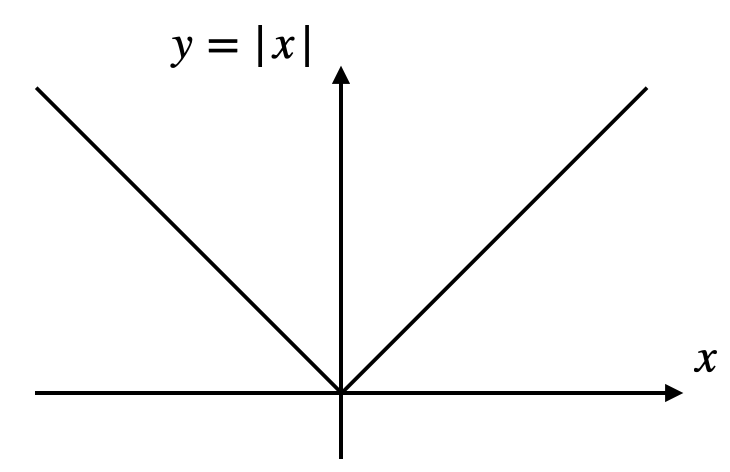
\includegraphics[width=50mm]{calculus4/abs.png}
 \end{center}
\end{figure}

直感的には, $0$で接線が引けないからである. 

\end{frame}


%%%%%%%%%%%%%%%%%%%%%%%%%%%%%%%%%%%%%%%%%%%%%%%%%%%%%%%%%%%%%%%%%%%%%%%%%%%%%%%%%%%%%%%
%%%%%%%%%%%%%%%%%%%%%%%%%%%%%%%%%%%%%%%%%%%%%%%%%%%%%%%%%%%%%%%%%%%%%%%%%%%%%%%%%%%%%%


\begin{frame}
\frametitle{導関数の非存在}


$f(x)=|x|$が$0$で微分不可能であることを確かめる. 
極限
$$
\lim_{h\to 0} \frac{f(a+h)-f(a)}{h}
$$
が存在すれば, 右極限と左極限
$$
\lim_{h\to +0} \frac{f(a+h)-f(a)}{h}, \ \ \ \lim_{h\to -0} \frac{f(a+h)-f(a)}{h}
$$
が存在して, それらは等しいはずである. 
そこで$a=0$とすると
\begin{align*}
\lim_{h\to +0} \frac{f(0+h)-f(0)}{h} & = 
\lim_{h\to +0} \frac{|h|-0}{h}=\lim_{h\to +0} \frac{h}{h}=1 \\
\lim_{h\to -0} \frac{f(0+h)-f(0)}{h} & = 
\lim_{h\to -0} \frac{|h|-0}{h}=\lim_{h\to +0} \frac{-h}{h}=-1
\end{align*}
であるから, 右極限と左極限は一致しない. 
\end{frame}



%%%%%%%%%%%%%%%%%%%%%%%%%%%%%%%%%%%%%%%%%%%%%%%%%%%%%%%%%%%%%%%%%%%%%%%%%%%%%%%%%%%%%%%
%%%%%%%%%%%%%%%%%%%%%%%%%%%%%%%%%%%%%%%%%%%%%%%%%%%%%%%%%%%%%%%%%%%%%%%%%%%%%%%%%%%%%%


\begin{frame}
\frametitle{導関数の計算}


\begin{Prob}
$(3x^2+5)(x^3+x)$の導関数を(1)展開してから計算, (2)積の微分公式を用いて計算, の2通りで求め, 答えが一致することを確かめよ. 
\end{Prob}


\begin{Prob}
$\frac{1}{x}$, $\frac{1}{x^2}$, $\frac{1}{x^3}$の導関数を計算せよ. 
\end{Prob}

\begin{Prob}
$\frac{x}{x+1}-(x+1)(x^2-4)$の導関数を計算せよ. 
\end{Prob}


\end{frame}


%%%%%%%%%%%%%%%%%%%%%%%%%%%%%%%%%%%%%%%%%%%%%%%%%%%%%%%%%%%%%%%%%%%%%%%%%%%%%%%%%%%%%%%
%%%%%%%%%%%%%%%%%%%%%%%%%%%%%%%%%%%%%%%%%%%%%%%%%%%%%%%%%%%%%%%%%%%%%%%%%%%%%%%%%%%%%%


\begin{frame}
\frametitle{定理\ref{微分定理}(2)の証明 (発展)}

公式$(f(x)g(x))'=f'(x)g(x)+f(x)g'(x)$を証明する. 
$$
(f(x)g(x))' = \lim_{h \to 0} \frac{f(x+h)g(x+h)-f(x)g(x)}{h}
$$
であり, 
\begin{align*}
& \frac{f(x+h)g(x+h)-f(x)g(x)}{h} \\
=& 
\frac{f(x+h)g(x+h)-f(x)g(x+h)}{h}
+
\frac{f(x)g(x+h)-f(x)g(x)}{h} \\
=& 
\frac{f(x+h)-f(x)}{h}g(x+h)
+
f(x)\frac{g(x+h)-g(x)}{h} \\
& \hspace{-4mm} \xrightarrow{h \to 0} 
f'(x)g(x)+f(x)g'(x). 
\end{align*}

\end{frame}



%%%%%%%%%%%%%%%%%%%%%%%%%%%%%%%%%%%%%%%%%%%%%%%%%%%%%%%%%%%%%%%%%%%%%%%%%%%%%%%%%%%%%%%
%%%%%%%%%%%%%%%%%%%%%%%%%%%%%%%%%%%%%%%%%%%%%%%%%%%%%%%%%%%%%%%%%%%%%%%%%%%%%%%%%%%%%%


\begin{frame}
\frametitle{定理\ref{微分定理}(3)の証明 (発展)}

公式$\Big(\frac{f(x)}{g(x)}\Big)'=\frac{f'(x)g(x)-f(x)g'(x)}{g(x)^2}$を証明する. 
$$
\Big(\frac{f(x)}{g(x)}\Big)'= \lim_{h \to 0} \Big(\frac{f(x+h)}{g(x+h)} - \frac{f(x)}{g(x)}\Big) \frac{1}{h}
$$
であり, 
\begin{align*}
&\Big(\frac{f(x+h)}{g(x+h)} - \frac{f(x)}{g(x)}\Big) \frac{1}{h} \\
=& 
\frac{f(x+h)g(x)-f(x)g(x+h)}{g(x+h)g(x)} \frac{1}{h} \\
=& 
\Big(
\frac{f(x+h)g(x)-f(x)g(x)}{h}- \frac{f(x)g(x+h)-f(x)g(x)}{h}
\Big) \frac{1}{g(x)g(x+h)}
\end{align*}

\end{frame}


%%%%%%%%%%%%%%%%%%%%%%%%%%%%%%%%%%%%%%%%%%%%%%%%%%%%%%%%%%%%%%%%%%%%%%%%%%%%%%%%%%%%%%%
%%%%%%%%%%%%%%%%%%%%%%%%%%%%%%%%%%%%%%%%%%%%%%%%%%%%%%%%%%%%%%%%%%%%%%%%%%%%%%%%%%%%%%


\begin{frame}
\frametitle{定理\ref{微分定理}(3)の証明 (発展)}


\begin{align*}
=& 
\Big(
\frac{f(x+h)-f(x)}{h} g(x)- f(x)\frac{g(x+h)-g(x)}{h}
\Big) \frac{1}{g(x)g(x+h)}
\\
& \hspace{-4mm} \xrightarrow{h \to 0} 
\frac{f'(x)g(x)-f(x)g'(x)}{g(x)^2}
\end{align*}

別証明として, 比較的簡単な$\Big(\frac{1}{g(x)}\Big)'=-\frac{g'(x)}{g(x)^2}$をまず示し, 
次に積の微分公式を$\frac{f(x)}{g(x)}=f(x) \frac{1}{g(x)}$に使うことで証明することも出来る. 

\end{frame}


%%%%%%%%%%%%%%%%%%%%%%%%%%%%%%%%%%%%%%%%%%%%%%%%%%%%%%%%%%%%%%%%%%%%%%%%%%%%%%%%%%%%%%%
%%%%%%%%%%%%%%%%%%%%%%%%%%%%%%%%%%%%%%%%%%%%%%%%%%%%%%%%%%%%%%%%%%%%%%%%%%%%%%%%%%%%%%%




\section{今日のまとめ}
\begin{frame}
\frametitle{まとめ}   


\begin{enumerate}
\item 平均変化率, 微分係数, 接線の傾き
\item 導関数, 導関数の性質
\end{enumerate} 


\end{frame}
